\documentclass[10pt]{article}
% for pdflatex
\usepackage[utf8]{inputenc}
% for hyperlink
\usepackage{hyperref}
\hypersetup{
    colorlinks=true,
    linkcolor=blue,
    filecolor=magenta,
    urlcolor=cyan,
}
% for custom enum
\usepackage{enumitem}
% for removing alinea begin of paragraph
\usepackage{parskip}
\usepackage{array, xcolor, graphicx}
\usepackage[a4paper, margin=1cm]{geometry}
\title{\bfseries\Huge Blockchain \& DevOps Engineer\vspace{-4ex}}
% no author
\author{\bfseries\Huge \vspace{-4ex}}
% no date
\date{}
% custom for column style
\definecolor{lightgray}{gray}{0.8}
% custom for column type
\newcolumntype{L}{p{0.18\textwidth}}
% custom for column type
\newcolumntype{R}{p{0.75\textwidth}}
% custom for column type
\newcommand\VRule{\color{lightgray}\vrule width 2pt}
% for bullet point outside of list
\newcommand{\tabitem}{~~\llap{$\rightarrow$}~~}
\begin{document}

\begin{minipage}[t]{0.80\textwidth}
\textbf{Mohamed Amine LEGHERABA}\\
26 years old\\
92 bis rue Rouget de Lisle, Bezons, France\\
\href{tel:+33630829000}{+33 6 30 82 90 00}\\
\href{mailto:mlegheraba@protonmail.com}{mlegheraba@protonmail.com}\\
\href{https://github.com/MohamedLEGH}{github.com/MohamedLEGH} \\

{\bf French}: native \\
{\bf Anglais}: fluent (TOIEC: 935) \\
\end{minipage}
\begin{minipage}[t]{0.20\textwidth}
\vspace{-3ex}
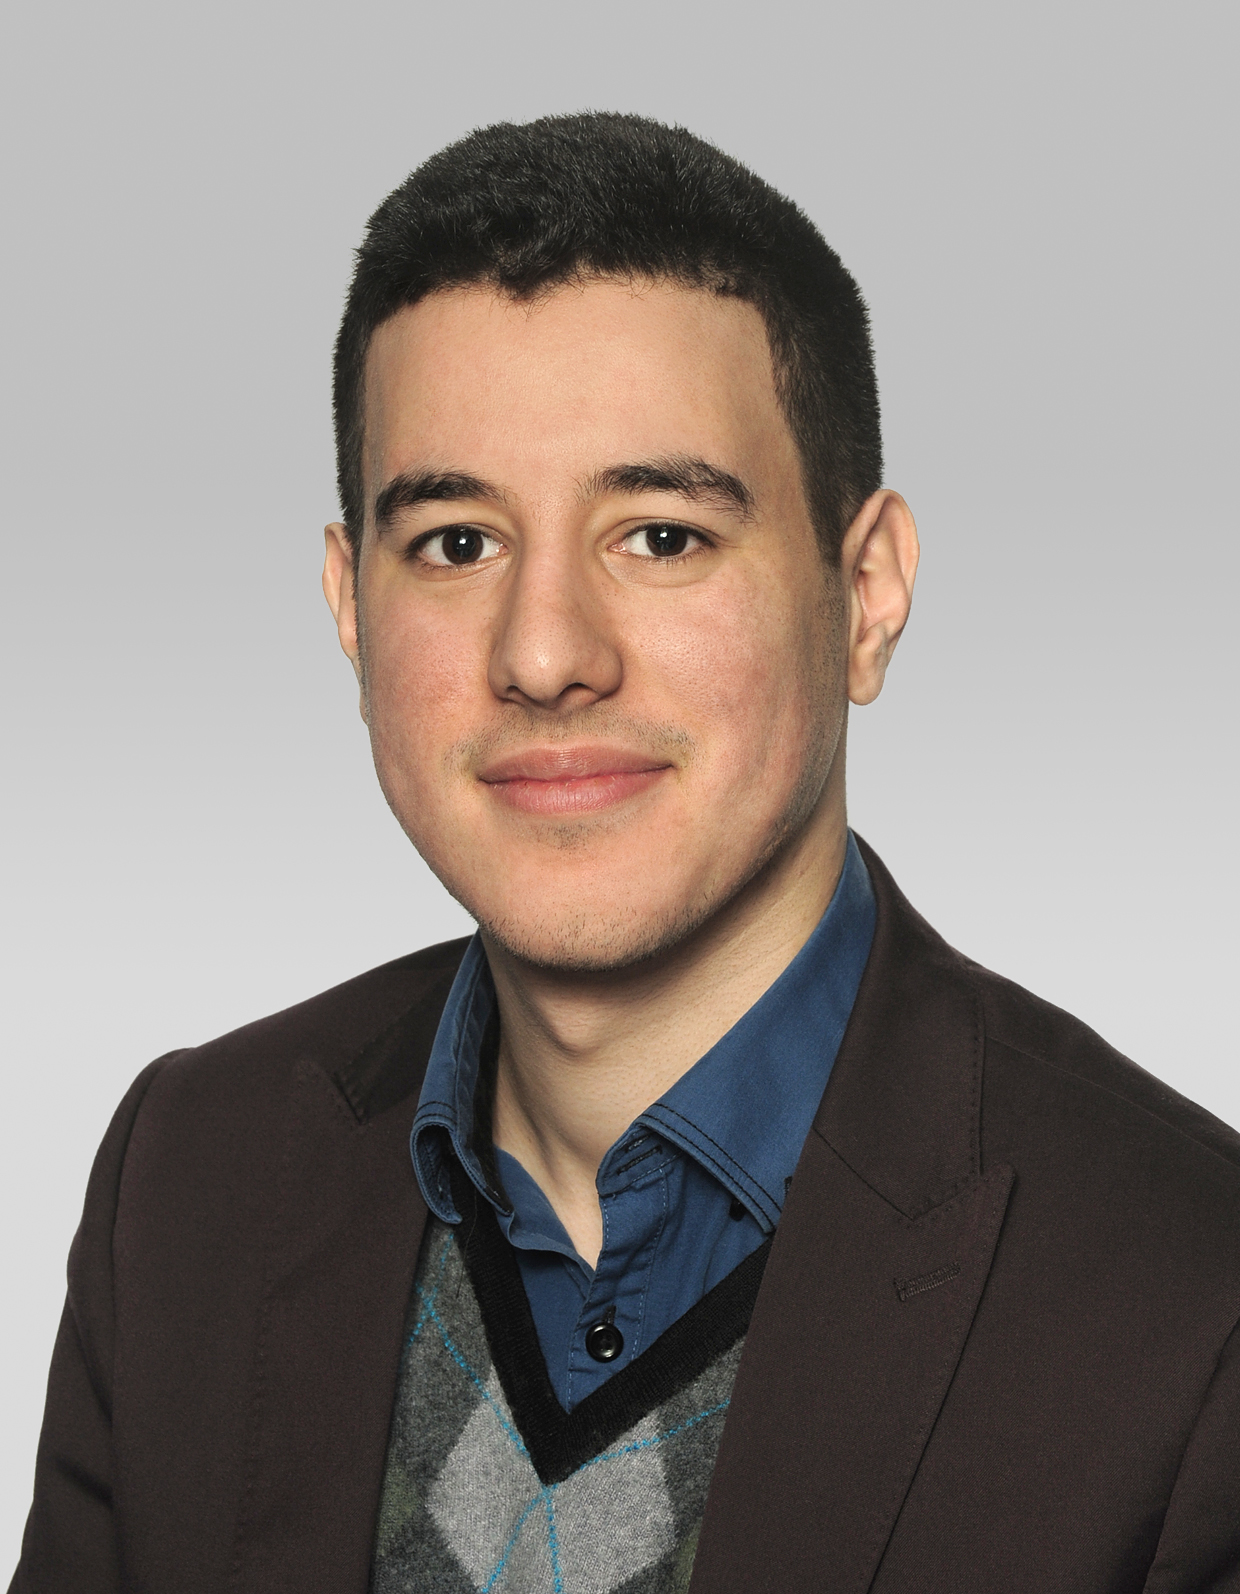
\includegraphics[width=3cm]{figures/Legheraba-Mohamed.jpg}
\end{minipage}
\vspace{-8ex}
% to make maketitle work without begin of page
{\let\newpage\relax\maketitle}
% to remove page number
\thispagestyle{empty}

\vspace{-8ex}

\section*{Formation}
\begin{tabular}{L!{\VRule}R}
\textbf{\textit{2015--2018}} & \textbf{Selective engineering school Polytech Sorbonne}, speciality \textit{Applied mathematics and computer science}. Erasmus semester at TU Delft, Netherlands, Winter 2017.\\[0.75cm]
\textbf{\textit{2013--2015}} & \textbf{Selective engineering school Polytech Sorbonne},  \textit{PeiP} (an intensive 2-year preparation course for the competitive
entrance to French engineering schools)\\[0.75cm]
\textbf{\textit{2013}}&\textbf{Secondary education leaving certificate}. In Science. With honours, Lycée Chaptal. \\
\end{tabular}


\section*{Work Experience}
\begin{tabular}{L!{\VRule}R}
\textbf{\textit{Since 2019}}& 
\includegraphics[width=2cm]{figures/SIA_logo.png} \hspace{0.2cm} {\bf Blockchain \& DevOps Engineer, Sia Partners} \\[0.25cm]

& \tabitem \small{\textbf{Development of blockchain applications for Sia Partners customers} (Banque de France experiments on CBDCs, Corda network for an asset manager, mobile payment application in cryptocurrencies, ...)}

\\[0.20cm]
& \tabitem \small{\textbf{Heka Project: \href{https://heka.sia-partners.com/en}{Software factory} for Data Science applications} (development of microservices in Python and React, continuous deployment on the Kubernetes infrastructure, ...)}

\\[0.20cm]
& \tabitem \small{\textbf{R\&D watch on blockchain, cryptocurrencies and distributed systems} (study of Liquid, Libra and TON blockchain networks, Lightning Network, HTLC Atomic Swap, Zero-knowledge proofs, Raft protocol, Taproot and Multi-Party Computation technologies, ...)}

\\[0.20cm]
& \tabitem \small{\textbf{Writing articles} (\href{https://www.sia-partners.com/fr/actualites-et-publications/de-nos-experts/la-blockchain-catalyseur-de-la-decentralisation-et-de-la}{\textit{Blockchain \& 5G}}, \href{https://www.sia-partners.com/fr/actualites-et-publications/de-nos-experts/entretien-avec-pierre-noizat-bitcoin-et-cryptomonnaies-0}{\textit{Interview with Pierre Noizat}}, ...)}

\\[0.20cm]
& \tabitem \small{\textbf{Course \textit{Programming a blockchain}} (\href{https://github.com/MohamedLEGH/tutoriel-blockchain-creation-bootstrap}{Polytech Sorbonne}, \href{https://github.com/MohamedLEGH/tutoriel-blockchain-MinesBootstrap}{Mines St Etienne}, ...)}

\\[0.20cm]
\textbf{\textit{March--September 2018}}& 
\includegraphics[width=1.5cm]{figures/ofi-am.png} \hspace{0.2cm} {\bf Blockchain \& Cloud R\&D watch intern, Development Department, OFI AM, 6 mois}.\\

\end{tabular}


\section*{Competences}
\begin{tabular}{ l l }
\textbf{Blockchain}: Ethereum, Corda, Hyperledger, Bitcoin & \textbf{DevOps}: Kubernetes, Gitlab CI/CD, GCP, Terraform \\[0.1cm]
\textbf{Smart contracts}: Solidity, Corda contrats, Chaincodes & \textbf{Tools}: Shell, Git, Docker, VS Code, PowerPoint \\[0.1cm]
\textbf{Mathematics}: Cryptography, Statistics, Graphs & \textbf{Programming}: Python, JavaScript, Bash, C/C++, Kotlin, R \\[0.1cm]
\textbf{Databases}: PostgreSQL, MySQL, SQLAlchemy & \textbf{Frameworks}: ReactJS, Node.js, Ethers.js, Flask, Web3.py, PyQt \\[0.1cm]
\textbf{Protocols}: Lightning Network, IPFS, TCP/IP & \textbf{Methodology}: Agile Method, APIs REST, Microservices \\[0.1cm]
\end{tabular}

\section*{Volunteer Experience}
\begin{tabular}{L!{\VRule}R}
\textbf{\textit{Since 2018}} & Association \textbf{Le Trait D’Union}, Homework help for high school and college students. Writing grant applications, treasurer. \\[0.75cm]

\textbf{\textit{2014--2017}} & Student association \textbf{Averroès}, Food donations for students, treasurer then president. \\
\end{tabular}
\section*{Interests}
\hspace*{1ex} \textbf{Electronics} (retrogaming console with a Raspberry Pi, fan control using a transistor, ...) \\
\hspace*{1ex} \textbf{Study of socio-economic doctrines} (liberalism, Austrian school of economics, anarchism, technoethics, ...) \\
\end{document}
